%------------------------------------------------------------------------------
% Preamble
%------------------------------------------------------------------------------

% File: anonymous-submission-latex-2025.tex
\documentclass[letterpaper]{article} % DO NOT CHANGE THIS

%\usepackage[submission]{aaai25}  % Remove authors and affiliations
\usepackage{aaai25} % Include authors and affiliations

% Might not be okay???
\usepackage{amsmath}
\usepackage[dvipsnames]{xcolor}
\usepackage{enumerate}

\definecolor{blue}{RGB}{47, 103, 177}
\definecolor{red}{RGB}{191, 44, 35}

\usepackage{times}  % DO NOT CHANGE THIS
\usepackage{helvet}  % DO NOT CHANGE THIS
\usepackage{courier}  % DO NOT CHANGE THIS
\usepackage[hyphens]{url}  % DO NOT CHANGE THIS
\usepackage{graphicx} % DO NOT CHANGE THIS
\urlstyle{rm} % DO NOT CHANGE THIS
\def\UrlFont{\rm}  % DO NOT CHANGE THIS
\usepackage{natbib}  % DO NOT CHANGE THIS AND DO NOT ADD ANY OPTIONS TO IT
\usepackage{caption} % DO NOT CHANGE THIS AND DO NOT ADD ANY OPTIONS TO IT
\frenchspacing  % DO NOT CHANGE THIS
\setlength{\pdfpagewidth}{8.5in} % DO NOT CHANGE THIS
\setlength{\pdfpageheight}{11in} % DO NOT CHANGE THIS
% These are recommended to typeset algorithms but not required. See the subsubsection on algorithms. Remove them if you don't have algorithms in your paper.
\usepackage{algorithm}
\usepackage{algorithmic}
% These are are recommended to typeset listings but not required. See the subsubsection on listing. Remove this block if you don't have listings in your paper.
\usepackage{newfloat}
\usepackage{listings}
\DeclareCaptionStyle{ruled}{labelfont=normalfont,labelsep=colon,strut=off} % DO NOT CHANGE THIS
\lstset{%
	basicstyle={\footnotesize\ttfamily},% footnotesize acceptable for monospace
	numbers=left,numberstyle=\footnotesize,xleftmargin=2em,% show line numbers, remove this entire line if you don't want the numbers.
	aboveskip=0pt,belowskip=0pt,%
	showstringspaces=false,tabsize=2,breaklines=true}
\floatstyle{ruled}
\newfloat{listing}{tb}{lst}{}
\floatname{listing}{Listing}
% Keep the \pdfinfo as shown here. There's no need
% for you to add the /Title and /Author tags.
\pdfinfo{
/TemplateVersion (2025.1)
}
\setcounter{secnumdepth}{0} % May be changed to 1 or 2 if section numbers are desired.
% Reduce hyphenation
\hyphenpenalty=2000

%------------------------------------------------------------------------------
% Meta-Data
%------------------------------------------------------------------------------

\title{Speeding up Narrative Planning with Causal Width Search and Pruning}

\author{
    Gage Birchmeier and Stephen G. Ware
}
\affiliations{
    Narrative Intelligence Lab\\
    University of Kentucky\\
    gage.birchmeier@uky.edu, sgware@cs.uky.edu
}

\begin{document}

\maketitle

%------------------------------------------------------------------------------
% Abstract and Links
%------------------------------------------------------------------------------

\begin{abstract}
Narrative planning can be used to create structured interactive experiences that dynamically respond to user input. Narrative planning works by generating a sequence of actions that achieves an author's desired goal while ensuring that there is an explanation for why each character takes each action in the sequence. An action in a sequence is considered necessary to that sequence if leaving the action out would prevent a later action in the sequence from being taken or prevent an author or character goal from being achieved. Using this definition, we define the causal width of a sequence to be the number of causally unnecessary actions, and we hypothesize sequences with a lower causal width are more likely to lead to a solution. We show that using causal width as a ranking mechanism can sometimes improve blind search, and ignoring stories with a high causal width can always improve the performance of heuristic search on a set of story benchmark problems.
\end{abstract}

% \begin{links}
%   \link{Code}{https://github.com/sgware/sabre-benchmarks}
% \end{links}

%------------------------------------------------------------------------------
% Content
%------------------------------------------------------------------------------

\section{Introduction}

Interactive narrative systems play a critical role in many pieces of media in domains such as entertainment and education. Interactive stories in virtual environments adapt to the user's choices. When an interactive narrative has some intended structure, such as a particular conclusion to the experience or constraints on which content must appear, the story needs to be planned either by a human author or automatically.

Narrative planning algorithms are one way to create structured interactive narrative. They take a set of characters, actions they can perform, and facts about the world that can be manipulated, then create a plan of actions that achieve some goal set by the author \cite{young2013plans}. Narrative planning is effective for introducing structure to a story as it defines a clear list of instructions to get from one world state to the next. One requirement for using these planning algorithms in real time is that they must be fast; otherwise, a user may be left waiting and become disengaged. We believe that one way to speed up narrative planning is to guide the planner in picking actions that become necessary for the full story to happen.

One important structural element of narratives is the causal dependencies that different events have on each other. We say that a later event is causally dependent on an earlier event when some outcome of the earlier event establishes a condition needed by the later event. We can further say that an event is \textit{causally necessary} to a story when leaving it out makes it impossible for some future event to occur.

We can think of the \textit{causally unnecessary} actions in a story as the ones that haven't yet been used for anything, structurally speaking. We hypothesize that prioritizing stories with a low number of causally unnecessary actions will help story planners find solutions faster. We tested two new methods of prioritizing a low number of unnecessary actions on a set of 14 benchmark storytelling problems \cite{ware2023collection}. First, we tested a new search technique that ranks stories by the number of causally unnecessary actions. This method only strictly improves on breadth-first search in two domains. Next, we tested a method of pruning stories with a high number of causally unnecessary actions during heuristic search. We found this pruning technique always improves search, allowing the planner to find more solutions and find them faster. We conclude this paper with a discussion of the performance of our techniques and areas for further research.

\section{Related Work}

\subsection{Causality in Narratology and Cognitive Science}

The importance of causality has long been recognized as an important element of story structure by narratologists \cite{chatman1993reading,bal1997narratology}. The effect of causality on narrative comprehension and mental modeling has also been widely studied in cognitive science~\cite{trabassosperry1985causal,gerrig1993experiencing,zwaan1998situation}.

Cognitive scientists distinguish several kinds of causality~\cite{tapiero2002mental}. For the purposes of this paper, we are discussing causality as \textit{enablement}. We say that an earlier event $A$ enables a later event $B$ just when $A$ establishes some effect which is needed by $B$. $A$ enables $B$ to occur, and $B$ could not occur without $A$; however $A$ does not necessarily force $B$ to occur---i.e. is possible that $A$ occurs and $B$ does not.

\subsection{Causality in Interactive Drama}
One defining feature of interactive fiction is that the player feels as if their actions impacted what happened afterward. Marlinspike is an interactive drama system that achieves this by creating stories such that the player's actions are necessary to the story \cite{tomaszewski2011use}. By doing so, the system produces stories that incorporate more of the player's significant actions, and doesn't leave them as unimportant. Similarly, our techniques prioritize stories that leave as few unimportant actions as possible.

\subsection{Causal Necessity in Narrative Planning}
Our definition of \textit{causal necessity} extends a definition previously developed for narrative planning by Ware, Senanayake, and Farrell (\citeyear{ware2023causal}). Under their definition, an action in a narrative is deemed necessary if and only if leaving it out of the plan would cause future actions to be impossible. Their work explored a cost function for search that discounted actions that were deemed to be causally necessary, in the hopes that stories with a higher number of causally necessary actions would be more likely to lead to a solution. This cost function had mixed results, improving search in only some benchmark problems.

This paper explores new techniques to improve narrative planning using a similar definition of causal necessity. Rather than discounting actions found to be necessary, we focus on the quantity of causally unnecessary actions within a plan as a trait of a story. Our goal is to limit the number of unnecessary actions in a story. We do so by implementing both a blind search strategy that expands stories with fewer unnecessary actions first and a pruning method for heuristic search that does not expand stories with too many unnecessary actions.

\subsection{Iterated Width Search}
Previous work in traditional planning has explored defining a sense of the \textit{width} of a plan, and using the width as a ranking or pruning function during search \cite{geffner2012width}. This enables search without a heuristic and improves heuristic search. With some modifications, width-based search can be competitive with state-of-the-art heuristic-based search \cite{lipovetzky2017best}. Our method of search is inspired by, but not directly based on, this idea of width-based search and pruning.

\section{Motivation}

Consider the example interactive narrative planning problem
introduced with the Sabre narrative planner, referred to as the \textit{Save Gramma} problem \cite{ware2021sabre}. The player starts in their cottage with
one coin and a quest to get a potion and return home. There
is a market where a merchant who wants money is selling
the potion and a sword for one coin each.
A bandit is waiting at a nearby camp. Their goal is to get as many coins as possible through any means necessary.
An armed guard is
stationed at the market to punish criminals. A crossroads connects the cottage,
market, and camp. Characters can walk between locations,
give an item to another character, buy an item from the
merchant, attack another character if they are armed, and
take items from slain characters. The story ends when the
player completes their quest by returning home with the
potion or dies.

The author's utility function is 1 when the player is dead, 2 when the player is at home with the potion, and 0 in all other states. This means the planner will accept any story where the player succeeds on their quest or dies trying, but it prefers stories where the player succeeds.

A search can also define a minimum acceptable author utility. For example, we can solve this problem with a desired utility of 1, which will accept any story where the player succeeds or fails. We can also set the desired utility to 2, which will only accept stories where the player succeeds.

Consider the potential solutions to this problem. Several actions can happen first: any character can walk to the crossroads, the guard can attack the merchant, and the merchant can give items away to the guard.
Suppose the first event in the story is that the player walks
to the crossroads. The state changes, but the list of actions
with satisfied preconditions remains about the same. The
options for where the player can walk have changed, but
otherwise the same set of actions remains possible: other
characters can walk to the crossroads, the guard can attack
the merchant, and the merchant can give items away to the
guard. The planner’s options for the second action in the
story are very similar to its options for the first action.

A human storyteller looking at this problem would
probably choose a second action that builds on the first.
Otherwise, what was the point of the first action? A planner,
however, has no such intuition, and it would consider any of
the available second actions an equally good choice. Each
choice represents a new branch in the search, quickly leading
to the combinatorial explosion that prevents narrative
planning from scaling to large problems. By incentivizing
action sequences with fewer unnecessary actions, we
hope to encourage the planner to reuse its past actions.

\section{Causal Width in Plans}

\subsection{Forward State-Space Planning}
We define our method in the context of forward state-space
planning, which builds a solution by adding one fully ground action at a time to the end of a plan. This puts our search in the space of fully ground, totally ordered sequential plans, built from start to finish.

Let the state space of a problem be a directed
graph whose vertices are states. An edge $s_1 \xrightarrow{a} s_2$ exists from
state node $s_1$ to state node $s_2$ and is labeled with action $a$
if and only if action $a$ can be taken in state $s_1$ and doing so
would change the state to $s_2$. Actions have preconditions that define when they can occur and effects that define how they change the state. Our method does not depend on any particular model of how these preconditions and effects work as long as it is possible, for any state $s$ and action $a$, to determine whether $a$ is possible in $s$.

Search begins in the initial state $s_0$ and follows edges
forward until it reaches an acceptable terminal state. A
classical planner simply defines a goal proposition; any state
where that proposition holds is an acceptable terminal state,
and any path from $s_0$ to a terminal state is a valid plan
\cite{russellnorvig}.
For narrative planning, rather than use a proposition, we use a utility function.

Narrative planners typically place additional constraints
on which paths are considered valid solutions. Requirements
differ by planner, but they typically define some model of
believable character behavior and require that the path to the
problem’s goal be composed only of believable actions. We
use the Sabre narrative planner \cite{ware2021sabre} in our
experiments. Sabre’s model of believable character behavior
reasons about intentionality and character beliefs. When a
character takes an action, the action is believable if and only
if it can be the first action in a plan the character believes
will improve their personal utility.
Our definition of causal necessity does not rely on Sabre’s
particular model of believability, so for details we refer
readers to the full description of that planner \cite{ware2021sabre}.
Though we tested our method in Sabre, our method can apply to non-narrative forward planners used for
storytelling \cite{porteous2010applying} and other
forward narrative planners like IMPRACTical \cite{teutenberg2015incorporating} and HeadSpace
\cite{sanghrajka2022headspace}
which use different definitions of believability.

\subsection{Causal Necessity}
Let $\pi$ be a sequence of $n$ actions $\{a_1, a_2, \ldots, a_n\}$. Let $\alpha(\pi, s)$ denote the state of the world if we begin in state $s$ and then
take each action in $\pi$ in that order. $\alpha(\pi, s)$ is defined if and
only if, for all $0 < i \leq n$, the edge $s_{i-1} \xrightarrow{a_i}s_i$ exists in the
state space. In other words, $\alpha(\pi, s)$ is defined if $\pi$ is a valid
path through the state space that starts at state $s$.

We define a \textit{causally necessary} action to be one that satisfies either of the following two conditions:
First, the action, if left out of the plan, makes at least one future action in the plan impossible.
Second, a character or author considers an action causally necessary if leaving it out leads to a lower utility than keeping it in.

Consider some sequence of actions $\pi=\{a_1,a_2,\ldots,a_n\}$ and some action $a_i$ in $\pi$ where $i \leq n$. Let $\pi'$ be the same sequence of actions with $a_i$ left out. In other words, $\pi'=\{a_1,\ldots,a_{i-1},a_{i+1},\ldots,a_n\}$.

We say that $a_i$ is causally necessary to the plan $\pi$ that starts in state $s$ by the first condition if $\alpha(\pi',s)$ is undefined. In other
words, if it is left out of the sequence, the actions that remain
no longer form a valid path from the state the plan starts in. 

Let $U(s)$ be the overall story utility value (called the \textit{author utility}) of state $s$. Let $U(c,s)$ be the utility of character $c$ in state $s$.

We say that $a_i$ is causally necessary to plan $\pi$ for the author by the second condition if $U(\alpha(\pi',s_0))<U(\alpha(\pi,s_0))$. We say that $a_i$, is causally necessary to plan $\pi$ that starts in state $s$ for character $c$ by the second condition if $U(c,\alpha(\pi',s))<U(c,\alpha(\pi,s))$. In other words, the author or character considers an action necessary if its inclusion in the plan raises their utility.

For a sequence of actions $\pi$, we define the \textit{causal width} of $\pi$ to be the number of actions that are \textit{not} causally necessary. The name \textit{causal width} parallels the definition of the ``width" of a plan or planning domain defined by Lipovetzky and Geffner in the paper that inspired this work \cite{geffner2012width}.  One can imagine a plan with more unused actions as being “wider”, with our hypothesis being that “narrower” plans are more likely to lead to a solution.

%Sometimes, an action may increase the authors utility, but not enough to bring it to our desired utility. In some domains with higher utility requirements, this can cause the planner to generate very lengthy plans leading up to one utility raising action that does not bring it high enough. To combat this, we present two choices of modification to our definition.

%Recall that the second condition for causal necessity states that the author considers an action necessary if leaving it in the plan raises their utility. For the first modification, we amend this condition by stating that if $\mu$ is the desired author's utility, $U(\alpha(\pi,s_0)) \geq \mu$ must also hold. That is, the desired author's utility must also be met by leaving the action in the plan.

%To illustrate this, consider a modified \textit{Save Gramma} problem where the author's utility was instead the number of coins the bandit has, and our desired utility is 3. The bandit starts with 0 coins. Consider a plan where the bandit kills the player, takes their coin, then kills the merchant, and takes the merchant's coin. We omit the walking actions the bandit must take for the sake of brevity, as they must all be necessary for the bandit to kill the player and the merchant in their respective locations. Killing the player and the merchant are necessary for the bandit to take their respective coins. Each time the bandit picks up a coin, the author's utility raises, but not enough to reach the desired amount. Thus by the first modification, these actions are currently unnecessary which gives this plan a causal width of 2.

%The second choice of modification is the following: When the author forms a plan that would have a causal width of 0 but does not improve the utility by the minimum amount, then we define the causal width to be 1 in that case to represent that at least one more action will need to be added to the sequence. In other words, for an author plan to have a causal width of 0, all actions must be necessary, and the plan must achieve the minimum required utility.

%Consider the previous example plan in the modified \textit{Save Gramma} problem. Each time the bandit picks up a coin their utility raises, making both of these actions necessary under this modification. However, this plan does not achieve the minimum desired author utility of 3. Thus, even though every action is considered necessary, this plan has a causal width of 1 under this modification.

% We display the results from using the second modification here in this paper. The second modification improved our results more than the first. In many domains, achieving a higher author utility requires achieving a lower author utility first. This is demonstrated in the modified \textit{Save Gramma} problem example. Giving plans that are closer to a solution a lower causal width helps the planner prioritize expanding that plan and find a full solution faster.

% When a character is forming a plan, if every action is causally necessary and the plan improves their utility, it has a causal width of 0. When considering a plan for the author (i.e., the story as a whole), we must also account for the search's minimum utility requirement. When the author forms a plan that would have a causal width of 0 but does not improve the utility by the minimum amount, then we define the causal width to be 1 in that case to represent that at least one more action will need to be added to the sequence. In other words, for an author plan to have a causal width of 0, all actions must be necessary, and the plan must achieve the minimum required utility.

\paragraph{Example}
To illustrate causal width, consider the following plan in the original \textit{Save Gramma} problem. This plan results in a state with author utility 2 as it ends with the player at home with the potion. This achieves the desired utility of 2 for this problem.

\begin{enumerate}[i]
  \item The player walks from their cottage to the crossroads
  \item The player walks from the crossroads to the market
  \item The player buys the potion
  \item The player walks from the market to the crossroads
  \item The player walks from the crossroads to their cottage
\end{enumerate}

Actions i, ii, and iv are causally necessary by the first condition. If the player does not first walk to the crossroads, they cannot then walk from the crossroads to the market. Note that the last action of any plan can never be causally necessary by the first condition since there are no actions after it.

Action v is causally necessary by the second condition. If it is left out of the plan, the player does not achieve their goal and thus does not increase their utility. Action iii is also necessary by the second condition. It can be left out of the plan without making any future actions impossible; however, if the player does not buy the potion, they have simply walked in a circle and have not completed their quest, and the plan will not improve the author's utility.

% Now consider another solution story with three actions.
% \begin{enumerate}[i]
%     \item The player walks from their cottage to the crossroads (intending to buy the potion, as above)
%     \item The bandit walks to their camp to the crossroads (intending to then take the player's money)
%     \item The bandit kills the player (intending to then take the player's money)
% \end{enumerate}

% Actions i and ii are causally necessary because the player and bandit need to be in the same place before the attack can happen. Action iii achieves an author utility of 1 because the player dies. If the search's minimum acceptable utility is 1, this story has a causal width of 0. If the minimum utility is 2, this story has a causal width of 1, because while it does increase the author's utility, it does not increase it enough.

\subsection{Using Causal Width During Search}
We examine two ways to use causal width during search. The first method is using the causal width of a plan as a ranking method for choosing which node in search to expand next, which we call \textit{Causal Width Search}. In this blind search technique, when selecting which node to expand next, we select one with the smallest causal width. This encourages the search to explore stories that contain mostly actions that build on each other.

The second method involves pruning nodes that have a causal width above a certain threshold, which we call \textit{Causal Width Pruning}. This method uses traditional heuristic search (like A*) but defines a cutoff width value $m$, such that any plan with a causal width greater than $m$ will not be expanded. We hope that by pruning plans with a high causal width, we can focus the planner's effort on expanding plans with actions that build off each other towards the goals of the characters and author.

\section{Causal Width Search}

Consider how a forward search would find the 5-action solution to \textit{Save Gramma}, which achieves an author utility of 2, discussed above: The player walks to the crossroads, then the market, purchases the potion from the merchant with their coin, then walks back to the crossroads, and finally home.

A traditional forward breadth-first search would expand all available plans of length 1 before any plans of length 2, and then all available plans of length 2 before any plans of length 3, and so on.

Causal Width Search instead expands all available plans with causal width 1 before expanding plans of causal width 2, then all available plans with causal width 2 before any with causal width 3, etc. When multiple plans have the same causal width, we break ties using the length of the story; so if two plans both have a causal width of 1, we would expand the shorter plan first.

Note that, unlike breadth-first search, expanding a story with causal width 2 might create a new story with a lower causal width of 1 or 0, which we will demonstrate here.

The planner constructs our solution to \textit{Save Gramma} one action at a time, so the first plan on the way to our example solution is simply the player walking from their home to the crossroads. Being the only action, it is also the last action, so it cannot satisfy the first condition of causal necessity. Walking to the crossroads does not increase the author's utility either, so this 1-action plan has a causal width of 1, meaning it has one action which does not yet have a clear structural purpose in the story.

The next plan on the path to this solution is for the player to walk from their house to the crossroads and then to the market. The player must be at the crossroads to walk to the market, so the first action has now become causally necessary. The second action is now the last and does not achieve our desired author's utility, so it is considered unnecessary. This 2-action plan also has a causal width of 1.

After walking to the crossroads and then to the market, the player buys a potion from the merchant with their coin. Both of the walking actions are now necessary to get the player to the market to buy the potion. Merely buying the potion does not achieve the author's goal as the player must also be at the cottage. Thus, the last action is still considered unnecessary, giving this 3-action plan a causal width of 1.

Once the player purchases the potion, they walk back to the crossroads. Again, the first two walking actions are necessary to get the player to the market so they can buy the potion. Buying the potion is still unnecessary, because leaving it out of the plan does not prevent the player from walking back to the crossroads, and without returning to the cottage, the author's utility has not yet improved. The last action of walking back to the crossroads is also unnecessary, so this plan then has a causal width of 2, meaning that two actions are currently not used.

The final plan is to have the player walk to the crossroads, then the market, buy the potion, walk back to the crossroads, and then walk back home. As always, the first two actions are necessary for the player to buy the potion. However, the author has now achieved the desired utility, as the player ends the story at home with the potion. This is not possible without the player purchasing the potion, so that purchase action is now considered necessary. The player walking from the market back to the crossroads and from the crossroads back home is now also necessary. All five actions in this plan are necessary, giving this final solution plan a causal width of 0.

Notice that the highest causal width we saw when building up to this plan was 2. This means that Causal Width Search will need to visit at least one node of width 2 before it can find a solution, and it will not visit any plans of width 2 until it has expanded all available plans of width 1 or less.

\subsection{The Endless Plans Problem}
One problem that arises during Causal Width Search is that there can be infinitely many plans that have a causal width of 1, which can make solving problems like \textit{Save Gramma} (which needs to expand at least one plan with causal width 2 to achieve a utility of 2)
impossible. This is because many domains have some way to make an infinite chain of actions that continue to build on each other. Consider a plan where the player walks to the crossroads, then walks home. The player walking to the crossroads is considered necessary as it allows the player to then walk from the crossroads back home, but walking home does not change the author's utility, so it is unnecessary (causal width 1). Imagine the player then walks back to the crossroads. Now the action of them walking from the crossroads back home is necessary, and only the final action is unnecessary (still causal width 1). This allows us to build an infinite loop of the player walking back and forth, and since each action is technically necessary for the next to occur, with the final action never changing the authors utility, there are infinite plans of the player walking back and forth between their home and the crossroads, all having a causal width of 1.

We observe that some states between the actions in these loops are identical. For example, the player walking to the crossroads and then back home changes nothing about the state of the world, creating a state that is identical to the initial state. Thus, we can prevent this infinite looping by introducing a new pruning condition. By pruning plans that contain duplicate states, we can prevent Causal Width Search from expanding infinite plans with causal width 1.





\subsection{The Causal Frontier}
To prune plans with duplicate intermediate states, we introduce the concept of the causal frontier and present an associated pruning strategy. A state node in the search space can determine the truth value of any proposition, such as ``The player is at the market'' and ``The merchant has the potion.'' A \textit{causal frontier} for a state $s_i$ where $i > 0$ is a conjunction of all atomic propositions that are true in $s_i$ but false in $s_0$, where $s_0$ is the initial state of the problem. For example, in the \textit{Save Gramma} domain, say the first action in a sequence is the player walking from their home to the crossroads. The causal frontier for the state after that action contains the proposition that the player is at the crossroads.

One of the features of Sabre is representing characters' beliefs about the state of the world, and these beliefs are part of the state. For example, after the player walks to the crossroads in the previous example, that player now believes their location is the crossroads. One of the issues that arises when modeling beliefs is that an infinite nesting of beliefs can occur. For example, the player also believes that the player believes that their location is the crossroads, and so on. There are an infinite number of belief propositions like this that would need to be included in the causal frontier.

To combat this issue, Sabre only keeps track of the beliefs that will be checked when planning. This includes any belief that is a precondition for an action or trigger, or a condition in a utility function. There is a finite number of these beliefs, along with a finite number of other possible propositions, which allows us to construct a finite representation of the causal frontier for states in Sabre. Other narrative planners that do not allow infinite theory of mind, like IMPRACTical \cite{teutenberg2015incorporating}, do not face this problem and can more easily calculate the causal frontier, or can simply detect and avoid plans that repeat the same state.

When analyzing a plan, we are particularly interested in whether two states after different actions in the plan share an identical causal frontier. Formally, this happens for a sequence of actions $\{a_0, \ldots, a_n\}$, starting from state $s_0$, when two actions $a_i, a_k$ for $0 < i < k \leq n$ result in intermediate states that share an identical causal frontier.

We also hypothesize that a solution can always be found from search without expanding a plan with a duplicate causal frontier. Consider states $s_a$ and $s_b$ after actions $a$ and $b$ in a plan where $a$ precedes $b$. If the causal frontiers of $s_a$ and $s_b$ are identical, we believe the actions between them can simply be discarded. This is because the actions after $s_b$ can still be performed starting from $s_a$, by our definition of the causal frontier. To illustrate this, consider a plan in the \textit{Save Gramma} problem where the player walks from their house to the crossroads, back home, then back to the crossroads, then to the market. The two times they walk to the crossroads result in two states with a duplicate causal frontier. They could have just walked to the market after the first time they walked to the crossroads.

By detecting and pruning plans that repeat a causal frontier, we fix the problem in Causal Width Search that allowed us to construct infinitely long plans with a causal width of 1. We can now evaluate whether the notion of causal width is helpful during search.

We acknowledge, however, that this method of pruning does not entirely solve the endless plans problem. This is due to the existence of unbound numeric fluents in states. Consider a change to the walk action in the \textit{Save Gramma} domain that gives the player a coin each time they take it. Now, walking in circles can be done infinitely, as there will never be a plan with duplicate intermediate frontiers, as the player's coin count will be different each time. In addition to causal frontier pruning, we imposed a limit on the length of a plan which mitigates this issue, but finding a better solution to the endless plans problem is a key direction for future work.

\begin{table*}[t]
\centering
\footnotesize
%\title{Comparison of planner performance across domains}

% \begin{tabular}{|c c | r r r | r r r r r |} 
% \hline
% \multicolumn{2}{|c|}{} & \multicolumn{3}{c|}{Breadth First Search} & \multicolumn{5}{c|}{Causal Width Search} \\
 
%  \hline
%  Domain & \shortstack{Desired \\Utility} & \shortstack{Times \\ Solved} & \shortstack{Nodes \\ Visited} & \shortstack{Time \\ (ms)} & \shortstack{Times \\ Solved} & \shortstack{Nodes \\ Visited} & \shortstack{Percent \\ Change} & \shortstack{Time \\ (ms)}  &  \shortstack{Percent \\ Change}\\ [0.5ex] 
%  \hline\hline
%  Bribery & 1 & 10 & 9.2 & 0.8 & 10 & 9.2 & 0\% & \textcolor{red}{1.1} & \textcolor{red}{+37.5\%} \\ 
%  \hline
%  Deer Hunter & 1 & 10 & 10,104.0 & 887.4 & 10 & \textcolor{red}{749,452.0} & \textcolor{red}{+3,984.4\%} & \textcolor{red}{486,925.6} & \textcolor{red}{+54,771.0\%} \\
%  \hline
%  Secret Agent & 1 & 10 & 662.6 & 6.0 & 10 & \textcolor{blue}{144.4} & \textcolor{blue}{-78.2\%} & \textcolor{red}{10.2} & \textcolor{red}{+70.0\%} \\
%  \hline
%  Hospital & 1 & 10 & 31,299.9 & 11,563.7 & \textcolor{red}{0} & \textcolor{red}{-} & \textcolor{red}{-} & \textcolor{red}{-} & \textcolor{red}{-}\\
%  \hline
%  Basketball & 1 & 10 & 1,349.0 & 561.0 & \textcolor{red}{0} & \textcolor{red}{-} & \textcolor{red}{-} & \textcolor{red}{-} & \textcolor{red}{-}\\
%  \hline
%  Fantasy & 1 & 10 & 4.0 & 1.8 & 10 & 4.0 & 0\% & \textcolor{red}{3.6} & \textcolor{red}{+100.0\%} \\
%  \hline
%  Fantasy & 2 & 10 & 7,469.0 & 2,670.0 & 10 & \textcolor{blue}{3,930.8} & \textcolor{blue}{-47.2\%} & \textcolor{red}{28,248.9} & \textcolor{red}{+958.0\%}\\
%  \hline
%  Fantasy & 3 & 0 & - & - & \textcolor{blue}{10} & \textcolor{blue}{5,120.7} & \textcolor{blue}{-} & \textcolor{blue}{7,857.9} & \textcolor{blue}{-}\\
%  \hline
%  Space & 1 & 10 & 4.0 & 1.1 & 10 & 4.0 & 0\% & \textcolor{red}{1.7} & \textcolor{red}{+54.5\%}\\
%  \hline
%  Space & 2 & 10 & 17.3 & 2.7 & 10 & \textcolor{red}{602.0} & \textcolor{red}{+3,379.8\%} & \textcolor{red}{440.3} & \textcolor{red}{+16,207.4\%} \\
%  \hline
%  Space & 3 & 10 & 17.3 & 6.5 & 10 & \textcolor{red}{602.0} & \textcolor{red}{+3,379.8\%} & \textcolor{red}{528.6} & \textcolor{red}{+8,032.3\%}\\
%  \hline
%  Space & 4 & 10 & 119.8 & 35.4 & 10 & \textcolor{red}{162.0} & \textcolor{red}{+35.2\%} & \textcolor{red}{149.8} & \textcolor{red}{+323.2\%} \\
%  \hline
%  Space & 5 & 10 & 866.9 & 197.5 & 10 & \textcolor{red}{4,431.5} & \textcolor{red}{+411.2\%} & \textcolor{red}{1,804.4} & \textcolor{red}{+813.6\%}\\
%  \hline
%  Raiders & 1 & 10 & 790.2 & 96.1 & 10 & \textcolor{red}{1,032.8} & \textcolor{red}{+30.7\%}& \textcolor{red}{556.4} & \textcolor{red}{+479.0\%} \\
%  \hline
%  Treasure Island & 1 & 10 & 50.0 & 0.6 & 10 & \textcolor{blue}{25.0} & \textcolor{blue}{-50.0\%} & \textcolor{red}{1.0} & \textcolor{red}{+66.7\%}\\
%  \hline
%  Save Gramma & 1 & 10 & 2,167.0 & 1,279.1 & 10 & \textcolor{red}{26,221.1} & \textcolor{red}{+1,110.0\%} & \textcolor{red}{22,095.3} & \textcolor{red}{+1,627.4\%}\\
%  \hline
%  Save Gramma & 2 & 10 & 11,391.2 & 7,501.2 & 10 & \textcolor{red}{252,593.3} & \textcolor{red}{+2,117.4\%} & \textcolor{red}{375,243.2} & \textcolor{red}{+4,902.4\%}\\
%  \hline
%  Jailbreak & 1 & 10 & 640.8 & 92.2 & 10 & \textcolor{red}{3,799.1} & \textcolor{red}{+493.0\%} & \textcolor{red}{1,909.3} & \textcolor{red}{+1970.8\%}\\
%  \hline
%  Jailbreak & 3 & 10 & 918,236.7 & 115,830.2 & 10 & \textcolor{blue}{14,249.5} & \textcolor{blue}{-98.4\%} & \textcolor{blue}{7,506.1} & \textcolor{blue}{-93.5\%}\\
%  \hline
%  Lovers & 1 & 10 & 1,349.0 & 561.0 & \textcolor{red}{0} & \textcolor{red}{-} & \textcolor{red}{-} & \textcolor{red}{-} & \textcolor{red}{-}\\  
%  \hline
% \end{tabular}

\begin{tabular}{|c c | r r r | r r r r r |} 
\hline
\multicolumn{2}{|c|}{} & \multicolumn{3}{c|}{Breadth First Search} & \multicolumn{5}{c|}{Causal Width Search} \\
 
 \hline
 Domain & \shortstack{Desired \\Utility} & \shortstack{Times \\ Solved} & \shortstack{Nodes \\ Visited} & \shortstack{Time \\ (ms)} & \shortstack{Times \\ Solved} & \shortstack{Nodes \\ Visited} & \shortstack{Percent \\ Change} & \shortstack{Time \\ (ms)}  &  \shortstack{Percent \\ Change}\\ [0.5ex] 
 \hline\hline
 
 Bribery & 1 & 10 & 9.2 & 0.1 & 10 & 9.2 & 0\% & \textcolor{red}{0.8} & \textcolor{red}{+700\%} \\ 
 \hline
 
 Deer Hunter & 1 & 10 & 10,104.0 & 760.5 & 10 & \textcolor{red}{348,713.0} & \textcolor{red}{+3,351.2\%} & \textcolor{red}{177,164.4} & \textcolor{red}{+23,195.8\%} \\
 \hline
 
 Secret Agent & 1 & 10 & 662.6 & 4.9 & 10 & \textcolor{blue}{134.4} & \textcolor{blue}{-79.7\%} & 4.9 & 0 \\
 \hline
 
 Hospital & 1 & 10 & 31,299.9 & 8,243.9 & \textcolor{red}{0} & \textcolor{red}{-} & \textcolor{red}{-} & \textcolor{red}{-} & \textcolor{red}{-}\\
 \hline
 
 Basketball & 1 & 10 & 1,349.0 & 29,936.6 & \textcolor{red}{8} & \textcolor{red}{886,053.1} & \textcolor{red}{2,859.8\%} & \textcolor{red}{1,779,604.9} & \textcolor{red}{5,844.6\%}\\
 \hline
 
 Fantasy & 1 & 10 & 4.0 & 0.9 & 10 & 4.0 & 0\% & \textcolor{red}{1.6} & \textcolor{red}{+77.7\%} \\
 \hline
 
 Fantasy & 2 & 10 & 7,469.0 & 2,349.0 & 10 & \textcolor{blue}{547.8} & \textcolor{blue}{-92.7\%} & \textcolor{blue}{1,017.1} & \textcolor{blue}{-56.7\%}\\
 \hline
 
 Fantasy & 3 & 0 & - & - & \textcolor{blue}{10} & \textcolor{blue}{5,099.7} & \textcolor{blue}{-} & \textcolor{blue}{182,646.9} & \textcolor{blue}{-}\\
 \hline
 
 Space & 1 & 10 & 4.0 & 2.1 & 10 & 4.0 & 0\% & \textcolor{blue}{0.7} & \textcolor{blue}{-66.7\%}\\
 \hline
 
 Space & 2 & 10 & 17.3 & 3.3 & 10 & \textcolor{red}{168.0} & \textcolor{red}{+871.1\%} & \textcolor{red}{128.0} & \textcolor{red}{+3,778.8\%} \\
 \hline
 
 Space & 3 & 10 & 17.3 & 2.5 & 10 & \textcolor{red}{168.0} & \textcolor{red}{+871.1\%} & \textcolor{red}{54.6} & \textcolor{red}{+2,084.0\%}\\
 \hline
 
 Space & 4 & 10 & 119.8 & 16.2 & 10 & \textcolor{red}{168.0} & \textcolor{red}{+40.2\%} & \textcolor{red}{54.7} & \textcolor{red}{+237.7\%} \\
 \hline
 
 Space & 5 & 10 & 866.9 & 129.4 & 10 & \textcolor{red}{5,699.2} & \textcolor{red}{+557.4\%} & \textcolor{red}{1,171.4} & \textcolor{red}{+805.5\%}\\
 \hline
 
 Raiders & 1 & 10 & 790.2 & 58.4 & 10 & \textcolor{red}{1,032.8} & \textcolor{red}{+30.7\%}& \textcolor{red}{223.4} & \textcolor{red}{+282.5\%} \\
 \hline
 
 Treasure Island & 1 & 10 & 50.0 & 0.5 & 10 & \textcolor{blue}{25.0} & \textcolor{blue}{-50.0\%} & \textcolor{blue}{0.3} & \textcolor{blue}{-40.0\%}\\
 \hline
 
 Save Gramma & 1 & 10 & 2,167.0 & 1,279.1 & 10 & \textcolor{red}{4,153.4} & \textcolor{red}{+91.7\%} & \textcolor{red}{4,536.0} & \textcolor{red}{+254.6\%}\\
 
 \hline
 Save Gramma & 2 & 10 & 11,391.2 & 6,490.4 & 10 & \textcolor{red}{284,735.2} & \textcolor{red}{+2,399.6\%} & \textcolor{red}{414,489.7} & \textcolor{red}{+6,286.2\%}\\
 \hline
 
 Jailbreak & 1 & 10 & 640.8 & 92.2 & 10 & \textcolor{red}{3,199.1} & \textcolor{red}{+399.2\%} & \textcolor{red}{937.3} & \textcolor{red}{+916.6\%}\\
 \hline
 
 Jailbreak & 3 & 10 & 918,236.7 & 269,147.1 & 10 & \textcolor{blue}{14,257.5} & \textcolor{blue}{-98.4\%} & \textcolor{blue}{4,523.0} & \textcolor{blue}{-98.3\%}\\
 \hline
 
 Lovers & 1 & 10 & 6,524.8 & 561.0 & \textcolor{red}{0} & \textcolor{red}{-} & \textcolor{red}{-} & \textcolor{red}{-} & \textcolor{red}{-}\\  
 \hline
 
\end{tabular}
\caption{This table compares the results of Breadth First Search (BFS) and Causal Width Search (CWS) search on each of our benchmark problems. Problems not solved by either planner are omitted. The Nodes Visited and Time columns are averages of the plans expanded and time taken, respectively, in each successful solve of each benchmark problem. Here, a greater Times Solved value indicates positive results, as it means the planner succeeded in solving the problem more often. A smaller Nodes Expanded or Time value indicates positive results as it means the planner was more efficient in solving the problem. Results from CWS that are better than BFS are shaded in blue, and worse results are shaded in red. Results for time are only considered better or worse when they deviate from BFS by more than $5\%$.}
\label{bfstable}
\end{table*}

\subsection{Causal Width Search Evaluation}

We first want to evaluate whether our simple Causal Width Search method can be effective on its own. We compared Causal Width Search to simple breadth-first search (BFS) on a suite of benchmark problems for the Sabre narrative planner \cite{ware2023collection}. 

For each problem, we put constraints on temporal depth, explanation depth, epistemic depth, and nodes visited. Temporal depth is the total number of actions that have occurred since the initial state. Explanation depth is the total number of actions that have occurred since the planner started attempting to explain a character's action. These constraints limit how long a story can be and how long a character's explanation of why they took an action can be, respectively. Epistemic depth limits how deeply nested theory of mind can go (what I believe you believe, and so on). We used the limits recommended by the benchmark problem documentation, which are the minimum values that allow all the known example solutions for each problem to be generated. All problems used a node limit of 1 million, meaning the planner was allowed to expand up to 1 million plans during its search for a solution. Each problem was run 10 times, and between each run, the list of actions in the problem was randomly shuffled to control for the influence of the arbitrary order in which actions are considered when expanding a plan.

There are several configurations of Sabre that could reasonably be called breadth-first search. We used a breadth-first search based on temporal depth. This means the length of a plan is measured as the number of actions that have occurred since the initial state. We compared this search to our Causal Width Search that we defined in the previous section. Causal Width Search uses Causal Frontier Pruning to avoid generating plans with loops, as discussed in the previous section.

\subsubsection{Results}

Table~\ref{bfstable} shows the results of comparing breadth-first search (BFS) to Causal Width Search (CWS). Overall, we found that using causal width as a ranking function is not better than BFS for most of the selected benchmarks. There were a few problems where CWS outperformed BFS. Two problems that were solvable by BFS were not solved by CWS, but there was one problem (\textit{Fantasy} with a minimum utility of 3) that was solved by CWS but not BFS.

\subsubsection{Discussion}

Causal Width Search generally did better on problems where the solution has a low causal width. Several of the benchmark problems have a structure where a motivating action needs to happen at the start of the story but does not become causally necessary until the end. For example, one solution to \textit{Deer Hunter} is for the protagonist to become hungry, then pick up and load a gun, hunt a deer, and eat it. The \textit{becomes hungry} action lowers the protagonist's utility and is needed to motivate all future actions, but it does not become causally necessary until the end of the story when he eats. The first action is causally unnecessary and remains so until the very end, meaning the story has a causal width of 2 for most of its duration until its causal width drops to 0. We discuss this further in the Limitations section at the end of the paper.

It is also notable that our implementation of Causal Width Search in many problems saw a significantly large percent change in the amount of time taken to solve a problem. This is because causal width needs to be calculated for every plan that is expanded. As can be seen from our definition of causal width, the calculation of it for a plan is in $O(n^2)$, and can be costly as plans get long. In scenarios where calculating causal width can reduce the amount of plans expanded, this can create a tradeoff between the amount of plans expanded and the amount of time taken. It is also worth noting that planning itself is PSPACE-hard, so the quadratic calculation of causal width will not dominate planning in large enough domains.

\begin{figure*}[!htb]
\centering
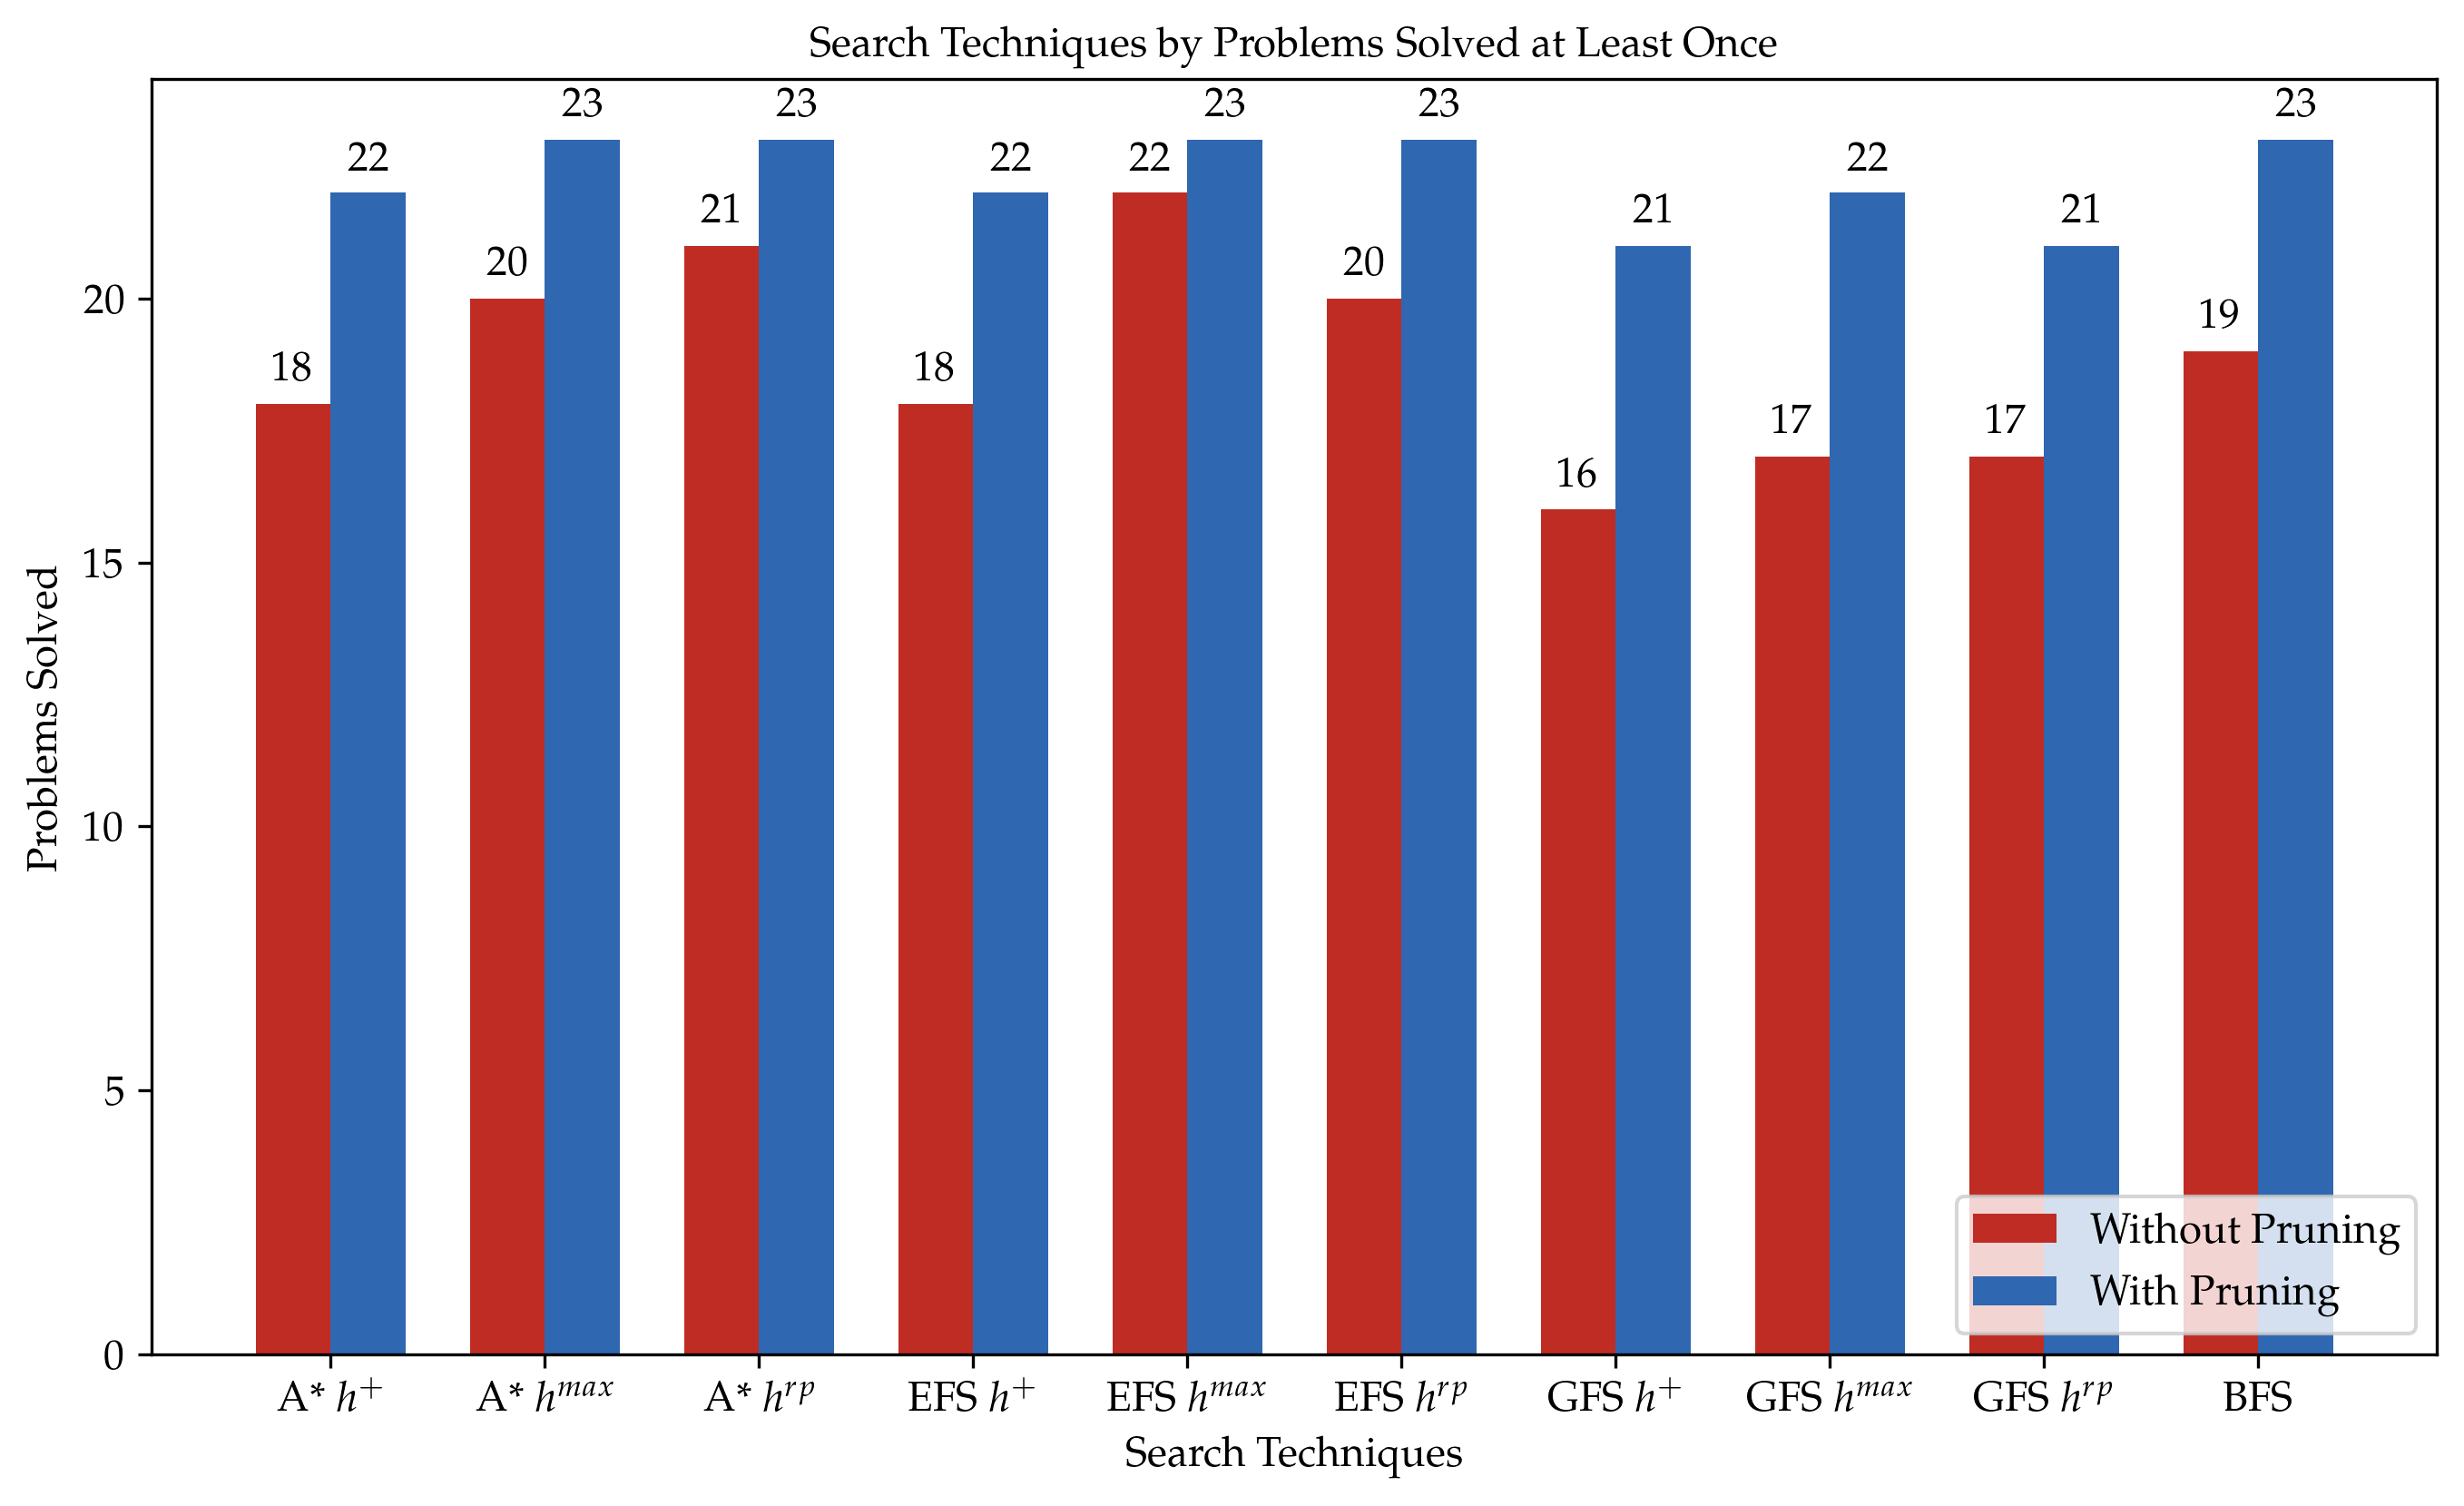
\includegraphics[width=0.95\textwidth]{plot1.png}
\caption{This graph shows, for each planner, the number of benchmark problems at solved least once under our constraints. The red bars represents the problems solved by each planner using its default configurations, and the blue bar represents the problems solved by each planner with the addition of Causal Frontier Pruning and Causal Frontier Pruning. Here, a taller bar indicates a positive result where the planner was able to solve a greater number of unique problems thanks to Causal Width Pruning and Causal Frontier Pruning.}
\label{probsolved}
\end{figure*}

\begin{figure*}[!htb]
\centering
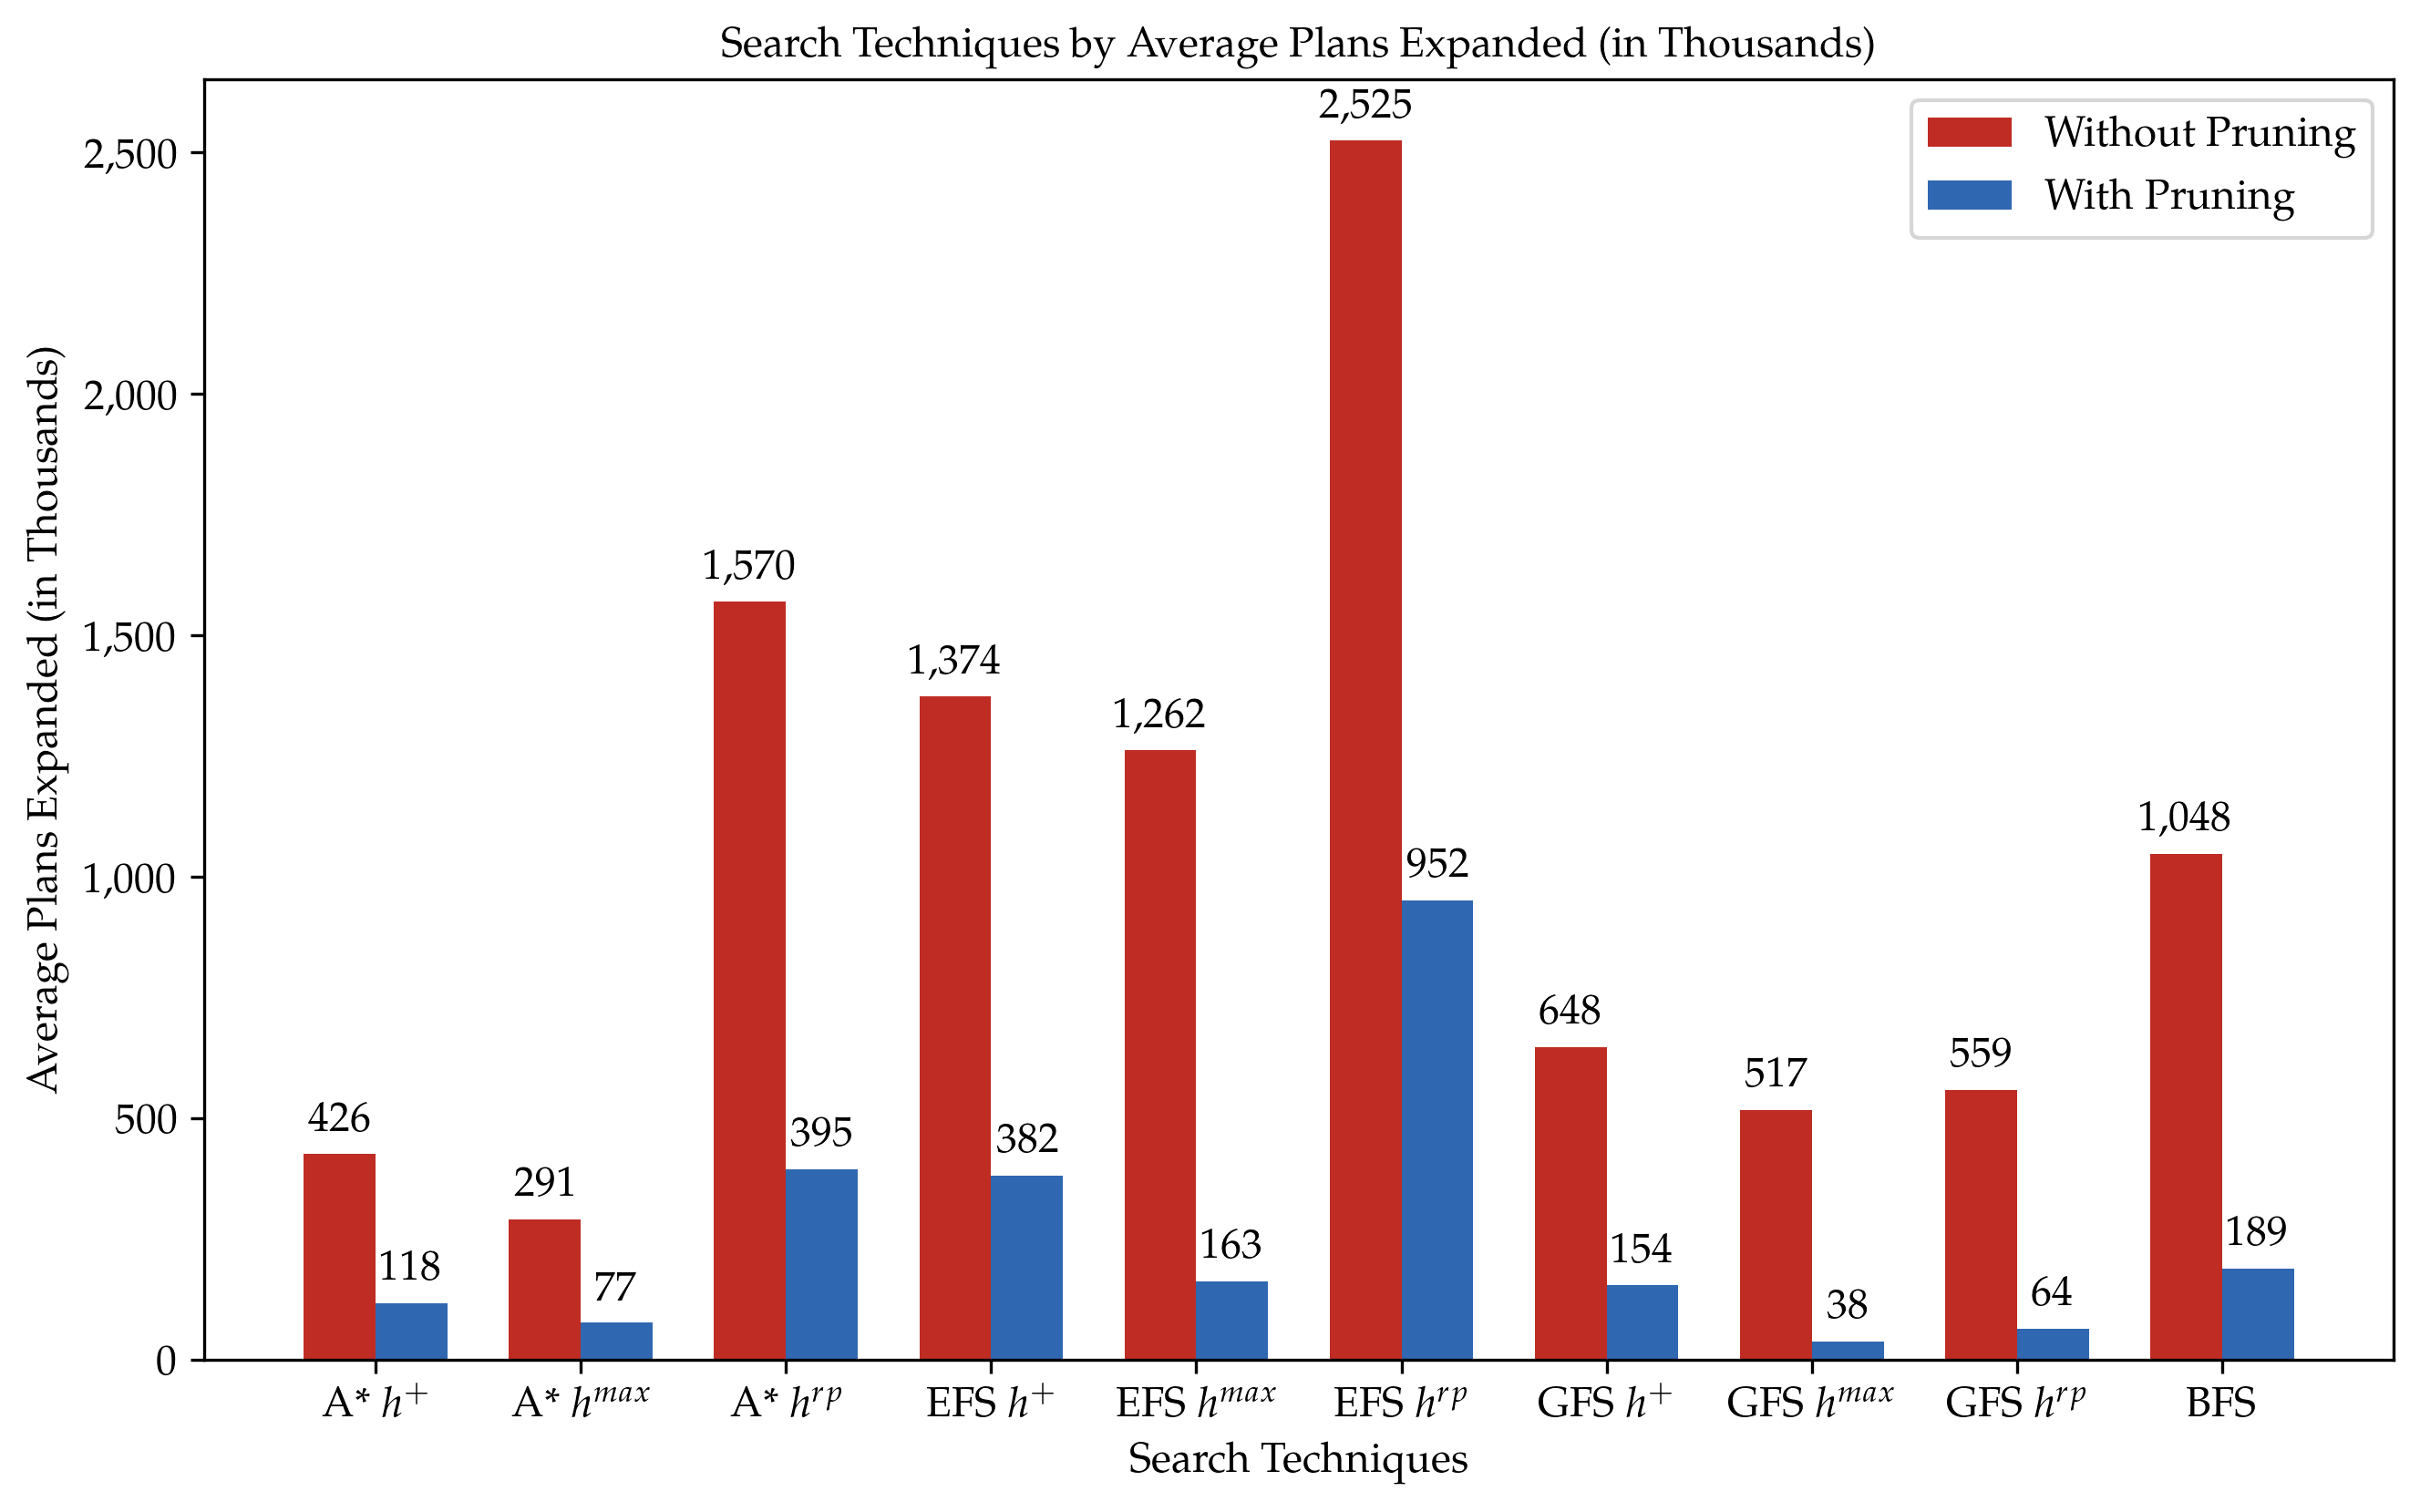
\includegraphics[width=0.95\textwidth]{plot2.png}
\caption{This graph shows, for each planner, the sum of the average number of plans expanded during search. The red bars represents the average number of plans expanded using its default configurations, and the blue bar represents the average number of plans expanded by each planner with the addition of Causal Frontier Pruning and Causal Frontier Pruning. For each combination of planner and its pruning counterpart, we only consider problems that were solved by both planners. Here, a shorter bar indicates a positive result where the planner was able to solve problems with fewer nodes expanded thanks to Causal Width Pruning and Causal Frontier Pruning.}
\label{avgnodes}
\end{figure*}

\subsection{Causal Width Pruning Evaluation}

Though causal width may not be effective on its own as a search strategy, we hypothesize that it can be used to improve existing heuristic search methods. Recall that Causal Width Pruning means setting a limit $m$ and not expanding any plans whose causal width exceeds $m$. We can also do Causal Frontier Pruning in addition to Causal Width Pruning, since it provides further improvements.

We tested our two pruning methods on nine configurations of heuristic search. We tested three search methods: A*, explanation-first search (EFS), and goal-first search (GFS). Explanation-first is similar to A* but requires an action to be fully explained before it can be added to a story. Goal-first requires the planner to verify that an action can contribute to achieving the goal before it attempts to explain it. A*, EFS, and GFS were each tested with three different heuristics: $h^+$, $h^{max}$, \cite{bonet2001planning} and the relaxed plan heuristic, which is similar to the Fast Forward heuristic \cite{hoffmann2001ff}, and which we refer to as $h^{rp}$. These three heuristics are well-known heuristics from the classical planning literature. As a baseline, we also include BFS in this evaluation. We compared the results of these ten search configurations to the results of those same searches but augmented with Causal Width Pruning and Causal Frontier Pruning.

We used the same limits on temporal depth, explanation depth, epistemic depth, and nodes visited as in the previous evaluation. Each problem was run 10 times, as in the previous evaluation. For each problem, we also need to put a limit on the causal width for pruning. We did this by measuring the minimum causal width required to find the example solutions to the benchmark problems given in their documentation.

We hypothesize that pruning plans above a causal width limit and with duplicate causal frontiers will improve the number of unique problems a planner can solve, and will decrease the number of nodes that it needs to visit.

\subsubsection{Results}

We saw an improved performance in two critical areas. First, as seen in Figure \ref{probsolved}, all techniques saw an increase in the number of problems they were able to solve at least once with the given constraints. In addition, when summing the total nodes visited by a planner in problems both the standard version and the pruning version were able to solve, we saw that the pruning version always visited fewer nodes. This is shown in Figure \ref{avgnodes}. However, we cannot draw many conclusions between different planners from this graph, since some different search and heuristic combinations solved different problems. The different bar sizes between different planners may mean numerous other things besides the effects of our pruning techniques. This includes indicating more problems solved, more difficult problems solved, or more nodes visited.

The results summarized in these two figures allow us to conclude that Causal Width and Duplicate Frontier Pruning are always able to improve the search techniques on our set of benchmark problems. The pruning allows heuristic planning to solve new problems and solve problems it could already solve with less effort.

\subsection{Discussion}

We demonstrated in Figure \ref{probsolved} that all heuristic searches could solve more problems under our constraints when paired with our pruning techniques. The new problems that could be solved often involved lengthy plans, around 7 to 9 steps in a solution, or they had many characters and actions that made the state space incredibly large. This may be because these long plans need to build off of previous actions many times which makes the Causal Width Pruning quite helpful.

The significant performance increase from Causal Width Pruning is due to the removal of unnecessary plans that are unlikely to lead to a solution. Many of the intended solutions of problems in our benchmark domains have actions that typically build off the immediately preceding action. Thus removing plans that deviate too far from this structure helps the planner find a solution with less plans expanded.

\section{Causal Width as a Heuristic}

During our investigation, we also tested a variant of A* search that uses temporal depth as the plan's cost and causal width as the heuristic. It did not yield any significant improvements over the other methods discussed above. We expect this is because causal width does a poor job estimating the amount of actions needed to create a valid solution. For example, in the \textit{Save Gramma} domain, the plan ``walk from the cottage to the crossroads'' and the plan ``walk from the cottage to the crossroads, walk from the crossroads to the market, buy the potion'' both have a causal width of 1. However, they need need 4 and 2 more actions respectively to reach an author utility of 2. In terms of plan length, a heuristic value of 1 is a poor estimate of the 4 remaining actions needed.

\section{Limitations}

We see three major limitations with our definition of causal width and how we used it in narrative planning. The first two limitations are flaws related to our definition of causal width. The third limitation stems from our method of Causal Width Pruning. 

First, our definition of causal necessity does not fully encapsulate the idea of an action being necessary to a story. To illustrate this, imagine that in the \textit{Save Gramma} problem the player did not know where they could obtain a potion. The author could still explore the same plan of the player walking over to the market, buying the potion, and returning home, but this story wouldn't be explained for the player, since they did not know it was possible to buy a potion from the merchant. Now, suppose there was an action where the player reads an ad at their home stating that there are potions for sale at the market. To the player, going to the market and buying a potion would only make sense if they took this action first. But to the author, and by our definition of causal necessity, there is no need for the player to read this ad to walk over to the market. This would make the action of reading the ad causally unnecessary by our definition, and would cause plans to have a higher causal width than similar plans in the original \textit{Save Gramma} problem. For example, walking to the crossroads, then the market has a causal width of 1 as we demonstrated earlier, but reading the ad, then walking to the crossroads, then the market has a causal width of 2 as we have yet to see a purpose for reading the ad or walking to the market.

In Causal Width Search, plans with a higher causal width take longer to get explored. The plan where the player reads the ad, then walks to the crossroads, and then the market would only get explored after the planner has exhausted every single possible plan with causal width 1, assuming that we are also pruning any plans with duplicate frontiers. We already need to expand at least one plan of causal width 2 for the \textit{Save Gramma} problem, but this same problem is present in other benchmarks and inflates the causal width necessary. With Causal Width Pruning, requiring a higher causal width simply means the pruning strategy is less effective, since a higher causal width limit means more plans, mostly bad, will be expanded.

Our second limitation comes from the higher causal width imposed by actions that are ``planted" early in a story. A ``planted" action is one that doesn't see its significance until much later in a story, it can be thought of as foreshadowing something that occurs later. Because these actions don't become significant until later, it is likely they will not be considered necessary by our definition of causal width when first introduced. Because ``planted" actions are likely to be unnecessary for some time while planning, they can inflate the causal width, which can cause the solution to take longer to be explored as described earlier. 

While our methods do not account for narrative necessity in its entirety, it is possible to detect it. Future work in this domain could potentially detect narrative necessity and use that to calculate a value similar to our definition of causal width to use the strategies presented here. 

The second limitation deals specifically with Causal Width Pruning. For this technique to be as effective as possible, a limit has to be known in advance. This requires knowing the necessary causal width for search to find a desired solution. For example, we have shown that if we want to get our ideal solution in the \textit{Save Gramma} problem, Causal Width Pruning must be set to a minimum of 2. Any less, and the search can not find a solution; any greater, and the pruning becomes less effective. This, however, is not too severe a limitation. Many authors, when designing domains, have example solutions in mind. These solutions can be used to find a causal width limit to use. In addition, many domains already have a somewhat low causal width. In our set of 14 benchmark domains, half of them only required a limit of 2, and the highest limit any of them required was 4. Thus, we suspect that somewhere between 2 and 4 may be a good limit for most domains.

\section{Conclusion}

Narrative planning must be fast to be used in real time. In this paper, we have defined a notion of causal width for narrative plans that counts the number of unnecessary actions in a plan and hypothesized that a plan with a lower causal width is more likely to lead to a solution. We tested this hypothesis in two different ways. First, we introduced Causal Width Search, which ranks plans by their causal width and has a search algorithm expand the plan with the lowest causal width. Testing this technique on a set of narrative planning benchmark problems showed that this method rarely performed better than breadth-first search. Next, we tested heuristic search using well-known search methods and heuristics with additional pruning of high causal width plans. We found that on our set of benchmark problems, this pruning was always able to improve the performance of search, in terms of problems solved within our limits and the number of plans expanded. 

There are a few opportunities for further investigation. First, we noted that there are infinitely many plans with causal width 1 possible in many domains because of the ability to make an infinite loop of actions. We proposed the causal frontier and a pruning strategy to remove plans with infinite loops to solve this issue. There may be a more effective way to prune these redundant plans. We also showed that our definition of causal necessity does not fully encapsulate an action's necessity in a story. One example of this is how an action may change the beliefs of a character to motivate them to take further actions. Future work could provide a stronger definition of necessity to improve the effectiveness of the techniques shown here. While our experiments were done with Sabre, it would be possible to implement a defintion of causal width and use our techniques in other narrative planners, like IPOCL \cite{riedl2010narrative}, Glaive \cite{ware2014glaive}, or IMPRACTical \cite{teutenberg2013efficient}. The definition is almost identical, but instead of ``has utility increased,” one would check ``has the goal been achieved.”

\section{Acknowledgements}

This material is based upon work supported by the U.S. National Science Foundation under Grant No. 2145153 and the U.S. Army Research Office under Grant No. W911NF-24-1-0195. Any opinions, findings, conclusions, or recommendations expressed in this material are those of the authors and do not necessarily reflect the views of the National Science Foundation or the Army Research Office.


%------------------------------------------------------------------------------
% Bibliography
%------------------------------------------------------------------------------

\bibliography{bibliography}

\end{document}
